\documentclass[a4paper,fleqn,numbers,doubleblind]{cas-dc}
\usepackage{amsmath,amssymb,array,booktabs,graphicx,lineno,tabularx,xurl}
\usepackage[numbers,sort&compress]{natbib}
\usepackage{hyperref}
\hypersetup{hidelinks}
\newcolumntype{Y}{>{\raggedright\arraybackslash}X}
\setlength{\emergencystretch}{3em}
\begin{document}
\let\WriteBookmarks\relax
\def\floatpagepagefraction{1}
\def\textpagefraction{.001}
\shorttitle{Evidence-Gated Knowledge-Graph Augmentation}
\shortauthors{Anonymous Authors}
\title[mode = title]{Provenance-Preserving Evidence-Gated Knowledge-Graph Augmentation for Auditable Entity--Relation Extraction}
\author{Anonymous Authors}
\begin{abstract}
Graph-augmented extraction can retrieve useful associations, but a retrieved
association is not necessarily a fact stated in the current sentence, and
fluent generators make it difficult to trace a predicted relation to its source
span and audit why it was accepted. We develop a provenance-preserving,
evidence-gated framework that separates graph-informed candidate generation
from output acceptance. A graph derived only from training annotations supplies
bounded concept and relation hints to QLoRA-adapted Qwen3-4B extractors;
deterministic span reconstruction, entity acceptance, and relation verification
then retain only source-linked, type-compatible assertions. Evaluation on ADE
and CoNLL04 uses a shared strict character-span protocol and reports the
underlying dataset distributions. The completed tests show that the
provenance-gated system improves relation F1 over its matched source-only
generator on both benchmarks and records explicit acceptance decisions. The
relation improvement persists in two additional training repetitions on both
datasets and after exact CoNLL04 train--test text overlaps are excluded,
although the CoNLL04 entity score does not improve. These findings support
controlled graph augmentation as an auditable extraction layer for human
review: the gates establish structural admissibility and source linkage and
record an explicit acceptance path for each assertion, without implying
universal accuracy dominance.
\end{abstract}
\begin{keywords}
entity and relation extraction \sep knowledge graph \sep provenance
\sep evidence grounding \sep adverse drug effects \sep selective prediction
\end{keywords}
\begin{highlights}
\item A provenance-preserving graph-context policy separates candidate generation from output acceptance.
\item Deterministic gates retain source-linked, type-compatible entity and relation assertions.
\item Relation-F1 gains persist across ADE, CoNLL04, repeated runs, and overlap sensitivity analysis.
\end{highlights}
% CAS constructs the separate highlights sheet in an intentionally wide
% internal box; keep that class-internal box from producing a false layout
% warning after the visible content has already been wrapped correctly.
\begingroup\hfuzz=124pt\maketitle\endgroup

\section{Introduction}
\label{sec:introduction}
Structured information extraction connects unstructured text to searchable
entities, typed relations, and downstream knowledge systems. In applications
related to safety, an extracted association must also be inspectable: users
need to know which mention was identified, which sentence supported the
relation, and which transformations produced the final assertion. Drug-related
adverse-effect extraction illustrates this requirement directly. A model that
recognizes a drug and an adverse effect but invents an association between them
can create a misleading record even when its output is syntactically valid.
General-domain extraction provides a complementary test of the same technical
issue across a broader set of entity and relation labels.

Neural entity and relation models provide effective approaches to the
recognition problem~\cite{li2022ner,eberts2020spert}. Generative models offer a
flexible alternative in which a common structured output format can be reused
across label inventories. However, fluent generation does not guarantee that
the predicted objects are supported by their input~\cite{ji2023hallucination}.
This distinction matters when extracted triples are inserted into a graph:
errors become available to later retrieval or reasoning stages, potentially
propagating beyond the sentence that generated them.

Knowledge graphs can contribute typed domain priors~\cite{hogan2021kg}, and
retrieval augmentation can expose those priors without requiring all knowledge
to be stored in model parameters~\cite{lewis2020rag}. Their use introduces a
specific authority problem. A relation observed in a training sentence may
suggest what to search for, but it does not establish that the same relation
holds in a new sentence. A training graph may also return an example's own
annotation or reveal content shared across data splits. The useful question is
therefore not only whether graph context increases recall, but whether its
eligibility and influence can be controlled and audited.

We address this problem with a staged architecture. Separate source-only,
exact-anchor, and high-recall graph-conditioned generators establish a matched
comparison of input conditions. A deterministic relation verifier checks
structural and source-evidence requirements. A complementary entity gate uses
agreement, source-matched anchors, or verified relation endpoints to accept a
subset of the graph-conditioned candidates. The final system combines the
accepted entities with verified relations whose endpoints survive. The
architecture uses existing representation and adaptation methods; its
contribution is their governed composition, not a new backbone or a new
optimization algorithm.

This paper concentrates on ADE~\cite{gurulingappa2012ade} and
CoNLL04~\cite{roth2004conll}. ADE supplies a drug-safety-related extraction
task with two entity labels and one relation label. CoNLL04 supplies a
general-domain control with four entity labels and five directed relation
labels. Both use English sentence-level inputs, making it possible to examine
the extraction and verification mechanisms without importing a long-document
windowing problem. They are trained and evaluated separately; this is not a
cross-dataset zero-shot transfer experiment.

The contributions are threefold:
\begin{itemize}
\item A provenance-aware graph-context policy that uses only training
annotations, excludes candidates supported only by the current example, and
clears graph hints for exact train/evaluation text overlaps.
\item A deterministic composition of source-span reconstruction, entity
selection, and relation verification that retains evidence-linked assertions
and records the reasons behind output decisions.
\item A reproducible two-benchmark analysis that combines split and label
statistics, uniform strict-span scoring, validation ablations, completed test
comparisons, and an exact-overlap sensitivity analysis.
\end{itemize}

\section{Related work}
\label{sec:related}
\subsection{Joint entity and relation extraction}
Entity recognition must resolve both mention boundaries and types; relation
extraction additionally depends on recovering the correct directed
endpoints~\cite{li2022ner}. Global consistency constraints have a long history
in this setting, including the formulation associated with the CoNLL04
benchmark~\cite{roth2004conll}. SpERT enumerates spans and jointly models
entities and relations using a pretrained transformer~\cite{eberts2020spert}.
It is a particularly relevant comparison because it performs the same joint
task without requiring a generative JSON interface. Our experiments retrain
SpERT from a clean base encoder on the same training partitions rather than
using a released task checkpoint that may already include development data.

Recent joint extractors explore complementary output representations. OneRel
casts extraction as fine-grained triple classification, UniRel unifies entity
and relation interactions, and set-prediction networks treat the output as an
unordered collection of relational tuples
\cite{shang2022onerel,tang2022unirel,sui2024setprediction}. Boundary-oriented
methods either assemble mention boundaries or learn them through regression,
whereas position-aware models emphasize endpoint structure and relation
representations
\cite{tang2022boundaryassembling,tang2023boundaryregression,chen2022positionaware,zhang2022positionaware}.
Global entity matching and span-based single-stage decoding provide further
ways to reduce pipeline error propagation
\cite{gao2023ergm,han2023spanbased}. These studies primarily improve the
extraction architecture; our focus is the provenance and acceptance policy
applied to generated candidates.

GLiNER and GLiREL provide label-conditioned alternatives for entity recognition
and relation classification~\cite{zaratiana2024gliner,boylan2025glirel}.
These models differ from locally fine-tuned generators in supervision,
pretraining, and output construction. We therefore report the implemented
train-calibrated pipeline as a named external baseline, not as an exhaustive
assessment of either model family. A same-backbone zero-shot generator further
separates the benefit of local adaptation from that of graph conditioning.

\subsection{Graph context and constrained generation}
Knowledge graphs represent typed entities and relations explicitly, while
retrieval augmentation uses selected records as model
context~\cite{hogan2021kg,lewis2020rag}. GenIE constrains generative information
extraction with a structured output space and entity/relation
catalogues~\cite{josifoski2022genie}. Unified Structure Generation similarly
maps heterogeneous information-extraction schemas to a common structured
generation formulation~\cite{lu2022uie}. Catalogue validity and source support
are different requirements: an admissible entity or relation may still not be
asserted in the current input. Our graph context is consequently treated as a
candidate prior whose eligibility depends on training provenance and local
source matching.

BGE-M3 supplies frozen text representations for semantic pattern
retrieval~\cite{chen2024bgem3}. It is neither a graph neural network nor a
jointly optimized component of the extractor. QLoRA enables compact adaptation
of the Qwen3 backbone~\cite{dettmers2023qlora,qwen2025qwen3}. Neither method
alone defines whether a candidate should enter the final assertion graph; the
proposed gates make that acceptance policy explicit.

\subsection{Evidence and safety-oriented knowledge construction}
Hallucination research distinguishes well-formed outputs from source-faithful
ones~\cite{ji2023hallucination}. In safety-related graph construction,
prompt-based processing of accident reports likewise illustrates the need to
trace generated knowledge back to its sources~\cite{liu2025llmaccidentkg}.
ADE offers a more controlled benchmark for a drug-safety-related relation
task~\cite{gurulingappa2012ade}. The present study uses its released relation
annotations to evaluate source-linked extraction and the implemented evidence
constraints.

\section{Method}
\label{sec:materials-methods}
\subsection{Task formulation}
\label{sec:method}
Let the annotated corpus be
\begin{equation}
\mathcal D=\{(x_i,\mathcal E_i,\mathcal R_i)\}_{i=1}^{N},
\label{eq:dataset}
\end{equation}
where $x_i$ is the deterministic single-space concatenation of the released
tokens, $\mathcal E_i$ is its entity set, and $\mathcal R_i$ is its directed
relation set. An entity mention is represented as
\begin{equation}
e=(b,u,y),\qquad x[b:u]=m,
\label{eq:entity}
\end{equation}
where $[b,u)$ is a character interval, $y$ is an entity label, and $m$ is the
copied mention text. A relation $r=(e_s,z,e_t)$ has typed directed endpoints
and relation label $z$. Source identifiers and evidence spans are stored with
these objects. Repeated strings at different offsets remain distinct mentions.
The character-span requirement in Equation~\eqref{eq:entity} prevents a
normalized name alone from receiving credit for the wrong occurrence.

For a bounded graph context $\mathcal C_i$, the extraction task is
\begin{equation}
f_{\theta}(x_i,\mathcal C_i)
=\bigl(\widehat{\mathcal E}_i,\widehat{\mathcal R}_i\bigr),
\label{eq:task}
\end{equation}
where both predicted sets must be reconstructed against $x_i$ before they can
be scored or accepted. Setting $\mathcal C_i=\varnothing$ recovers the
source-only input condition; nonempty context remains advisory and does not
bypass the evidence gates.

The imported benchmark assigns every relation the status \texttt{explicit}
and uses its source sentence as the evidence span. This representation keeps
each evaluated relation tied to a concrete source sentence and makes the
evidence path available for inspection.

\subsection{Framework overview}
Figure~\ref{fig:architecture} summarizes the implemented flow. SOE
(Source-Only Extraction), EAE (Exact-Anchor Extraction), and HRGE (High-Recall
Graph Extraction) are separately trained QLoRA adapters on the same Qwen3-4B
snapshot. SOE uses source text and the training-derived ontology without graph
hints. EAE receives conservative concept hints, while HRGE receives bounded
anchors, edge priors, and semantic relation patterns.

EVGE (Evidence-Verified Graph Extraction) applies the relation verifier to
HRGE. CFE (Conservative-Fusion Extraction) pairs accepted HRGE entities with
endpoint-filtered raw HRGE relations. PGE (Provenance-Gated Extraction) pairs
the same accepted entities with endpoint-filtered verified relations. These
three systems are deterministic post-processing variants, not additional
trained networks. In deployment PGE needs EAE and HRGE candidates; SOE is a
comparison branch and does not participate in fusion.

\begin{figure*}[t]
\centering
\includegraphics[width=\textwidth]{../figures/methodology_detailed_draft.pdf}
\caption{Detailed methodology used in this study. The figure shows the ADE and
CoNLL04 inputs, dataset-specific training knowledge graphs, the Transformer
attention block, the SOE/EAE/HRGE QLoRA adapter branches, and deterministic
evidence gates based on agreement, anchors, endpoints, relation validity, and
source evidence.}
\label{fig:architecture}
\end{figure*}

\subsection{Provenance-controlled graph context}
Each training graph stores mention strings, types, directed relations, and
the sentence identifiers supporting them. For a training sentence $d$, a
candidate is excluded if its only supporting provenance is $d$. Candidates
with other supporting sentences remain eligible; their stored aggregate
support statistics are not recomputed as a fully leave-one-out graph. This
distinction prevents interpreting the provenance policy as complete removal
of every contribution from the current example.

Formally, let $\mathcal G_{\rm tr}=(\mathcal V_{\rm tr},\mathcal A_{\rm tr})$
be the graph constructed from training annotations and let $\pi(c)$ denote the
set of training-sentence identifiers supporting a context item $c$. During
adapter training, the provenance-eligible pool for current training item $i$ is
\begin{equation}
\mathcal C_i^{\rm elig}
=\{c\in\mathcal C_i^{\rm raw}:\pi(c)\setminus\{i\}\neq\varnothing\}.
\label{eq:provenance-eligible}
\end{equation}
Evaluation identifiers are disjoint from training identifiers. Exact source-text
overlap is handled separately by the quarantine rule below, which clears the
entire context rather than treating duplicated text as independent evidence.

EAE uses type-balanced, exact-matching concept hints. HRGE uses three context
channels. First, source-matched anchors must pass type-purity and mention-form
filters. Second, a typed edge prior requires support outside the current
example and both endpoint strings in the current source. Third,
frozen BGE-M3 retrieves semantically related relation-pattern records. If
$\mathbf{H}$ contains normalized eligible record embeddings and
$\mathbf{q}$ is the normalized source embedding, retrieval scores are
\begin{equation}
\mathbf{s}=\mathbf{H}\mathbf{q},\qquad
\mathcal I=\operatorname{TopK}_{k}\{i:s_i\geq\tau\}.
\label{eq:retrieval}
\end{equation}
Equation~\eqref{eq:retrieval} ranks candidate context, not accepted facts.
The bounded retrieval limits and thresholds are fixed in the protocol artifact
rather than tuned on the test set. The prompt explicitly identifies retrieved
objects as hints. Exact-overlap
quarantine overrides retrieval and clears all graph context for the affected
evaluation sentences.

\subsection{Structured generation and span reconstruction}
The generator emits entity identifiers, copied text and types, plus relation
identifiers, directed endpoint references, types, and explicit status. It is
not asked to calculate source offsets. Deterministic expansion assigns copied
mentions to occurrences in the supplied sentence and reconstructs character
spans; unmatched strings and invalid references are recorded. This separates
language-model candidate generation from source-coordinate bookkeeping.

Inference uses the full supplied sentence and a fixed generation policy.
Failed jobs are represented by empty predictions, not removed from the
denominator. These experiments do not use annotation-guided rescue windows or
label-dependent sentence truncation.

\subsection{QLoRA adaptation and training objective}
All three generators use one-epoch QLoRA adaptation of the same frozen
Qwen3-4B backbone. Low-rank updates are applied to the attention and
feed-forward projections. For an adapted projection $\ell$, QLoRA parameterizes
the effective weight as
\begin{equation}
W_{\ell}=W_{\ell}^{(0)}+\frac{\alpha}{r}B_{\ell}A_{\ell},
\qquad \operatorname{rank}(B_{\ell}A_{\ell})\leq r,
\label{eq:qlora}
\end{equation}
where $W_{\ell}^{(0)}$ is the frozen quantized weight, $r$ is the adapter rank,
and $A_{\ell}$ and $B_{\ell}$ are the trainable low-rank factors.

Let $y_{1:T}$ denote the serialized target and let $\omega_t$ equal one for a
target token and zero for a prompt token. The optimized objective is
\begin{equation}
\mathcal L(\theta)
=-\frac{1}{\sum_{t=1}^{T}\omega_t}
\sum_{t=1}^{T}\omega_t
\log p_{\theta}(y_t\mid y_{<t},x,\mathcal C).
\label{eq:training-objective}
\end{equation}
Thus prompt tokens are excluded from the loss. The same dataset partition and
optimization configuration are used for all branches and repetitions; full
settings are retained in the artifact manifest rather than repeated in the
narrative.

\subsection{Provenance-aware candidate validation and fusion}
For each relation label $z$, training annotations define permitted source-type
and target-type sets $S_z$ and $T_z$. The implemented type constraint is
$y_s\in S_z$ and $y_t\in T_z$; it does not additionally require that every
specific source/target type pair has been observed together. With component
checks for valid references, label, endpoint types, explicit status, and source
evidence, the relation predicate is
\begin{equation}
V(r)=V_{\rm ref}(r)\land V_{\rm label}(r)\land V_{\rm type}(r)
\land V_{\rm status}(r)\land V_{\rm evidence}(r).
\label{eq:verifier-predicate}
\end{equation}
Here $V_{\rm evidence}$ requires valid evidence and both endpoint strings in a
common source-evidence span. The accepted relation set is
\begin{equation}
R_V=\{r\in R_H:V(r)=1\}.
\label{eq:verifier}
\end{equation}
The entity gate uses three Boolean signals:
\begin{equation}
 A(e)=A_{\rm agree}(e)\lor A_{\rm anchor}(e)\lor A_{\rm endpoint}(e).
\label{eq:accept}
\end{equation}
The corresponding accepted entity set is
\begin{equation}
E_A=\{e\in E_H:A(e)=1\}.
\label{eq:accepted-entities}
\end{equation}
Agreement means that EAE predicts the same case-folded, whitespace-normalized
text and type. Anchor support requires a same-type source-gated HRGE anchor.
Endpoint support means that the entity participates in a relation retained by
Equation~\eqref{eq:verifier}. The three signals in Equation~\eqref{eq:accept}
are complementary but not statistically independent; verified endpoints are
a rule-based signal, not a second human judgement. Duplicate normalized
text/type candidates are collapsed within the sentence. Relations are retained
only when both referenced entities survive:
\begin{equation}
F(R,E)=\{(e_s,z,e_t)\in R:e_s\in E\land e_t\in E\}.
\label{eq:endpoint-filter}
\end{equation}
The two output compositions are
\begin{equation}
G_{\rm CFE}=(E_A,F(R_H,E_A)),\qquad
G_{\rm PGE}=(E_A,F(R_V,E_A)).
\label{eq:composition}
\end{equation}
Equation~\eqref{eq:composition} makes the difference between raw-relation
fusion and verified fusion explicit. Accept/reject decisions are logged. A
retained relation satisfies the stated structural and source-linkage rules, and
the applied checks are recorded with the output for inspection.

\section{Experiments}
\label{sec:experiment}
This section describes the common experimental setup, reports the main
held-out comparison, and then examines training behavior, stability,
component effects, compliance, and split-overlap sensitivity.

\subsection{Experimental setup}
The experiments compare PGE with its matched source-only generator under a
common strict-span protocol and examine component effects, training behavior,
run-to-run stability, and exact-overlap sensitivity. The two-benchmark scope is
a focused retrospective analysis rather than a preregistered representative
sample of extraction domains. Model and gate settings were fixed before the
reported test evaluation, and two additional complete repetitions provide a
limited stability check.

\subsubsection{Datasets}
\label{sec:data}
We use the sentence-level ADE and CoNLL04 files distributed in SpERT format.
Counts refer to that preprocessed distribution rather than every sentence in
the original source corpora. CoNLL04 retains its supplied training,
development, and test partitions. The ADE files contain 3,845 training
sentences and 427 test sentences; a deterministic development slice of 384
sentences is removed from the supplied training pool, leaving 3,461 training
sentences. The slice is selected by a fixed identifier-based procedure, not by
validation performance. This is one fixed ADE split, not an average over the
multiple folds sometimes used in the literature.

Table~\ref{tab:data} gives counts recomputed from the exact imported artifacts.
The unit called a document in the software is one benchmark sentence, not a
whole medical case report or news article. Both datasets are English; the
results therefore support neither multilingual nor cross-lingual claims.
Published annotations are imported rather than locally re-annotated.

\begin{table*}[t]
\centering\small\setlength{\tabcolsep}{4pt}
\caption{Dataset inventory for the exact experimental partitions. Length is
the number of whitespace-delimited tokens in the reconstructed source text.}
\label{tab:data}
\begin{tabular}{llrrrr}
\toprule
Dataset & Split & Sentences & Entities & Relations & Mean length \\
\midrule
ADE & train & 3461 & 8717 & 5470 & 21.17 \\
ADE & validation & 384 & 996 & 627 & 21.82 \\
ADE & test & 427 & 1126 & 724 & 21.24 \\
CoNLL04 & train & 922 & 3377 & 1283 & 28.77 \\
CoNLL04 & validation & 231 & 893 & 343 & 30.27 \\
CoNLL04 & test & 288 & 1079 & 422 & 28.94 \\
\bottomrule
\end{tabular}

\end{table*}

ADE contains \textsc{Drug} and \textsc{Adverse Effect} entities and a single
\textsc{Adverse Effect} relation label. The imported endpoint convention is
\emph{adverse effect to drug}; we preserve it rather than reversing it to a
more intuitive drug-to-effect direction. CoNLL04 contains \textsc{Location},
\textsc{Organization}, \textsc{Person}, and \textsc{Other} entities, with
\textsc{Work For}, \textsc{Kill}, \textsc{Organization Based In},
\textsc{Live In}, and \textsc{Located In} relations.

Table~\ref{tab:labels} lists exact label counts for every partition. The single
ADE relation label eliminates inter-class relation confusion but does not
eliminate endpoint detection, direction, or false-pair errors. CoNLL04 has a
broader relation inventory and more heterogeneous entity roles. Consequently,
a higher aggregate F1 on ADE should not be interpreted as evidence that
drug-safety reasoning is inherently easier than general-domain reasoning; the
supervised extraction tasks differ in structure and size.

\begin{table*}[t]
\centering\small\setlength{\tabcolsep}{4pt}
\caption{Exact entity and relation annotation counts in the imported files.}
\label{tab:labels}
\begin{tabular}{lllrrr}
\toprule
Dataset & Kind & Label & Train & Validation & Test \\
\midrule
ADE & Entity & ADVERSE EFFECT & 4631 & 529 & 616 \\
ADE & Entity & DRUG & 4086 & 467 & 510 \\
ADE & Relation & ADVERSE EFFECT & 5470 & 627 & 724 \\
CoNLL04 & Entity & LOCATION & 1219 & 322 & 427 \\
CoNLL04 & Entity & ORGANIZATION & 616 & 170 & 198 \\
CoNLL04 & Entity & OTHER & 455 & 118 & 133 \\
CoNLL04 & Entity & PERSON & 1087 & 283 & 321 \\
CoNLL04 & Relation & KILL & 179 & 42 & 47 \\
CoNLL04 & Relation & LIVE IN & 330 & 91 & 100 \\
CoNLL04 & Relation & LOCATED IN & 247 & 65 & 94 \\
CoNLL04 & Relation & ORGANIZATION BASED IN & 271 & 76 & 105 \\
CoNLL04 & Relation & WORK FOR & 256 & 69 & 76 \\
\bottomrule
\end{tabular}

\end{table*}

The mean training lengths are 21.17 reconstructed tokens for ADE and 28.77 for
CoNLL04. Their test means are 21.24 and 28.94, respectively. The cumulative
distributions describe all three partitions rather than only the training set.
These lengths are descriptive whitespace-token counts, not Qwen tokenizer
counts. The largest observed reconstructed length is 97 for ADE and 118 for
CoNLL04 across the imported partitions.

Every imported sentence contains at least one annotated relation. The selected
benchmark files therefore do not measure false-positive behavior over a
deployment stream dominated by sentences with no relevant relations. We retain
the supplied benchmark composition and do not create additional negative
sentences for the reported tests.

Figure~\ref{fig:data-distribution} reports training-label proportions and
empirical cumulative sentence-length distributions for every partition.
CoNLL04 is consistently shifted toward longer sentences, whereas the train,
validation, and test curves within each dataset remain broadly aligned.

\begin{figure*}[t]
\centering
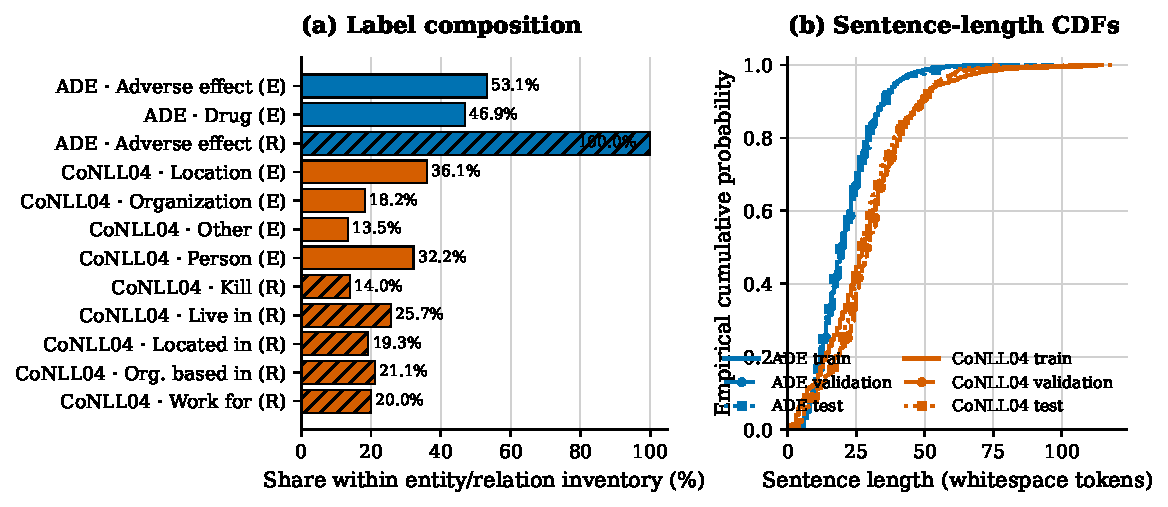
\includegraphics[width=\textwidth]{../figures/dataset_distribution.pdf}
\caption{Dataset distribution analysis. (a) Training-label composition within
each dataset's entity (E) or relation (R) inventory. Percentages sum to 100\%
separately within each dataset--kind combination. (b) Empirical cumulative
distributions of reconstructed sentence length for the train, validation, and
test partitions. Length is measured in whitespace-delimited tokens.}
\label{fig:data-distribution}
\end{figure*}

The graph is built separately for each dataset from its training annotations
only. An exact-overlap check compares case-folded source strings after
collapsing whitespace. ADE has no train/development or train/test exact-text
overlap under this check. CoNLL04 has 14 development sentences and 19 test
sentences whose text matches training content. For these sentences, both
exact-anchor and high-recall graph context are cleared before generation.

Clearing graph hints does not undo exposure of the trained generator to
duplicate training text. We therefore retain the supplied partitions for the
main comparison and report an additional fixed-prediction test analysis that
excludes the 19 overlapping CoNLL04 test sentences. We do not claim that the
benchmark is duplicate-cluster isolated or that this exact-match check detects
all near duplicates.

\subsubsection{Baselines and metrics}
The internal development comparison includes all six named systems. The test
table includes the two promoted systems and three completed external
comparisons. Qwen3-4B zero-shot uses the same backbone without local adapters,
followed by the recorded source expansion and relation verifier. SpERT is
trained from a base encoder on the same training partitions and its final
checkpoint is used without selecting a test-best epoch. GLiNER+GLiREL uses
predicted, not gold, entities and training-only calibration. Detailed baseline
hyperparameters are retained in the experiment artifacts. These are
heterogeneous baseline configurations, not equal-compute experiments.

All reported main-table predictions are rescored with one public
character-span evaluator. An entity key contains its exact source interval
and type. A relation key contains both typed directed entity keys and the
relation label. Predicted evidence offsets must resolve to the supplied source;
the evaluator does not recover missing offsets by searching normalized text.
Duplicate keys receive one vote, invalid objects remain unmatched predictions,
and omitted jobs remain empty. For pooled counts,
\begin{equation}
\begin{aligned}
P&=\frac{TP}{TP+FP},\\
R&=\frac{TP}{TP+FN},\\
F_1&=\frac{2TP}{2TP+FP+FN}.
\end{aligned}
\label{eq:metrics}
\end{equation}
Equation~\eqref{eq:metrics} is applied across sentences within each dataset,
not after averaging their individual F1 scores. Because all imported statuses
are explicit, claim-status-aware scores do not form a separate uncertainty
benchmark. The unified evaluator removes small denominator differences caused
by legacy duplicate handling; unchanged source artifacts and a reconciliation
report preserve the earlier metrics.

\subsubsection{Statistical analysis and compliance evaluation}
We compute paired bootstrap resamples of test sentences from fixed predictions
and recompute pooled F1 within each resample.
The percentile interval describes sentence-sampling uncertainty for the
completed model pair, not variability across training repetitions. Intervals are
descriptive, unadjusted for multiple comparisons, and are not used to change
the frozen models or gates.

For the two additional training repetitions, we report the arithmetic mean and sample
standard deviation of strict-span test F1. With only two repetitions, these
summaries show observed initialization sensitivity but do not reliably estimate
population variance. For the primary seed-42 EAE and HRGE adapters, the runner
log retains one loss observation every five optimizer steps. These observations
are matched to adapter metadata by run start time and are reported without
interpolating missing steps. The later repetitions retain only endpoint loss
summaries and are therefore excluded from the loss curves.

Evidence coverage and rule-invalid counts are measured separately from
extraction F1. These compliance counts refer to emitted prediction objects
before the evaluator's key deduplication. Exact-overlap sensitivity removes
the same affected test sentence identifiers from both systems, without
retraining or regenerating predictions. Test labels are used for reporting
statistics and scoring only, not for constructing graph hints or choosing
thresholds in this revision.

\subsection{Main results}
\label{sec:results}
Table~\ref{tab:test} reports the completed test results under the common
evaluator. PGE raises ADE relation precision from 80.62\% to 87.00\% and
recall from 67.82\% to 72.10\%, giving relation F1 of 78.85\% compared with
73.67\% for SOE. Entity F1 remains essentially unchanged, at 87.93\% versus
87.97\%. Thus, the main improvement is relational rather than a general gain
in mention recognition.

On CoNLL04, PGE raises relation precision from 54.61\% to 62.40\% and recall
from 56.16\% to 57.82\%. Relation F1 increases from 55.37\% to 60.02\%, while
entity F1 decreases from 83.83\% to 83.20\%. The composition trades some
entity coverage for a better relation precision--recall balance in this run.

\begin{table*}[t]
\centering\scriptsize\setlength{\tabcolsep}{2.6pt}
\caption{Completed test comparisons, strict source-character-span
micro scores (\%). Qwen3-ZS is Qwen3-4B zero-shot with the recorded verifier;
GLiNER+GLiREL uses training-only calibration. Each dataset uses its own test
partition. All rows are rescored with the same evaluator.}
\label{tab:test}
\begin{tabular}{llrrrrrr}
\toprule
Dataset & System & Ent. P & Ent. R & Ent. F1 & Rel. P & Rel. R & Rel. F1 \\
\midrule
ADE & Qwen3-ZS + verifier & 63.83 & 63.32 & 63.58 & 39.36 & 22.24 & 28.42 \\
ADE & GLiNER + GLiREL & 79.30 & 64.65 & 71.23 & 60.31 & 43.23 & 50.36 \\
ADE & SOE & 92.21 & $\mathbf{84.10}\uparrow$ & $\mathbf{87.97}\uparrow$ & 80.62 & 67.82 & 73.67 \\
ADE & PGE & $\mathbf{92.89}\uparrow$ & 83.48 & 87.93 & $\mathbf{87.00}\uparrow$ & $\mathbf{72.10}\uparrow$ & $\mathbf{78.85}\uparrow$ \\
CoNLL04 & Qwen3-ZS + verifier & 48.78 & 53.94 & 51.23 & 30.92 & 19.19 & 23.68 \\
CoNLL04 & GLiNER + GLiREL & 60.78 & 14.37 & 23.24 & 13.79 & 3.79 & 5.95 \\
CoNLL04 & SOE & 85.83 & $\mathbf{81.93}\uparrow$ & $\mathbf{83.83}\uparrow$ & 54.61 & 56.16 & 55.37 \\
CoNLL04 & PGE & $\mathbf{86.04}\uparrow$ & 80.54 & 83.20 & $\mathbf{62.40}\uparrow$ & $\mathbf{57.82}\uparrow$ & $\mathbf{60.02}\uparrow$ \\
\bottomrule
\end{tabular}

\end{table*}

Figure~\ref{fig:result-analysis} complements the exact values in
Table~\ref{tab:test}. It highlights that the matched PGE--SOE difference is
relation-specific: relation F1 increases on both datasets, whereas the entity
differences are close to zero and their paired intervals cross zero.

\begin{figure*}[t]
\centering
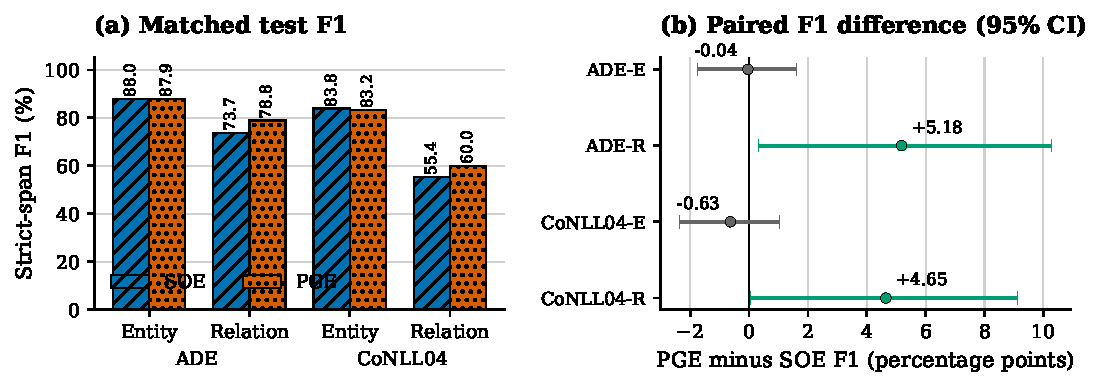
\includegraphics[width=\textwidth]{../figures/result_analysis.pdf}
\caption{Test-set analysis of the matched SOE and PGE systems. (a) Strict-span
entity and relation F1 on ADE and CoNLL04. (b) PGE-minus-SOE F1 differences;
horizontal intervals are paired 95\% sentence-bootstrap intervals from fixed
predictions. Exact values and all external baselines remain in
Table~\ref{tab:test}.}
\label{fig:result-analysis}
\end{figure*}

SpERT has the highest entity and relation F1 among these completed systems:
91.37\%/84.08\% on ADE and 89.02\%/69.72\% on CoNLL04. PGE therefore improves
the matched generative baseline but does not surpass this trained span-based
model. PGE also exceeds the recorded zero-shot and GLiNER+GLiREL pipelines on
both extraction tasks. The latter observation is specific to their implemented
label mapping and calibration; it is not a claim that every configuration of
those model families would perform worse.

\subsection{Training-loss diagnostics}
Figure~\ref{fig:training-loss} reports the recoverable seed-42 EAE and HRGE
training traces. The faint lines are the observations logged every five
optimizer steps; the emphasized lines are trailing means over ten logged
observations (50 optimizer steps). CoNLL04 shows a clear reduction over its
single epoch. ADE begins at a lower loss and remains noisy, with only a modest
late reduction; the trace should not be described as monotonically decreasing.
Because SOE and the additional repetitions do not have equivalently attributable
step histories, they are not mixed into this diagnostic.

\begin{figure*}[t]
\centering
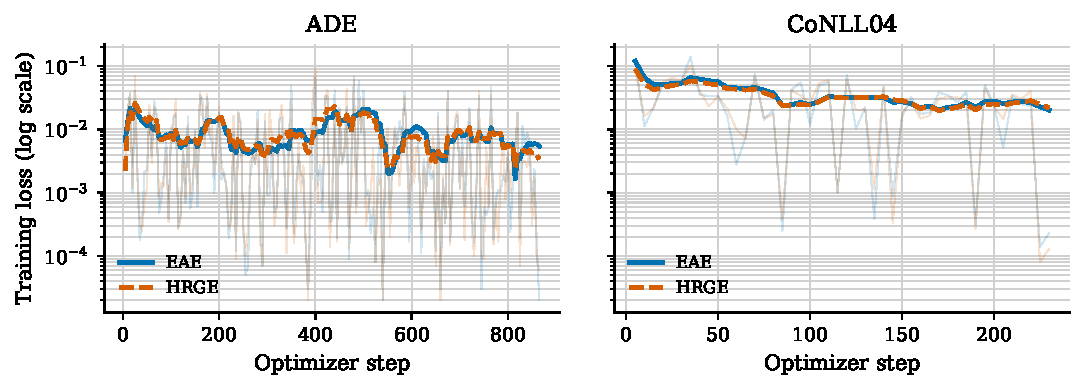
\includegraphics[width=\textwidth]{../figures/training_loss.pdf}
\caption{Audited seed-42 training loss for the EAE and HRGE adapters. Raw
observations (faint) were written to runner stdout every five optimizer steps;
emphasized curves are ten-observation trailing means. The logarithmic scale
retains the large variation in the raw observations. No intermediate values
are reconstructed or interpolated.}
\label{fig:training-loss}
\end{figure*}

\subsection{Additional-run stability}
Table~\ref{tab:repeated-runs} summarizes the two later repetitions. On ADE, PGE
improves relation F1 over SOE in both repetitions (81.20\% versus 78.31\%, and
80.62\% versus 78.06\%). On CoNLL04, the corresponding differences are positive
but smaller (58.50\% versus 56.91\%, and 61.45\% versus 60.92\%). Across the two
runs, the mean relation-F1 difference is 2.73 points on ADE and
1.06 points on CoNLL04. CoNLL04 entity F1 decreases by 0.51 points on average,
so this check supports a relation-specific rather than universal improvement.

\begin{table*}[t]
\centering\small\setlength{\tabcolsep}{4pt}
\caption{Test stability across two additional training repetitions under the common strict-span
evaluator (micro \%, mean $\pm$ sample standard deviation; $n=2$). The final
column is the mean PGE-minus-SOE relation-F1 difference.}
\label{tab:repeated-runs}
\begin{tabular}{llrrr}
\toprule
Dataset & System & Entity F1 & Relation F1 & $\Delta$ relation F1 \\
\midrule
ADE & SOE & $88.00\pm0.37$ & $78.18\pm0.18$ & -- \\
ADE & PGE & $89.35\pm0.04$ & $80.91\pm0.41$ & $+2.73$ \\
CoNLL04 & SOE & $82.26\pm1.91$ & $58.92\pm2.84$ & -- \\
CoNLL04 & PGE & $81.75\pm2.02$ & $59.98\pm2.09$ & $+1.06$ \\
\bottomrule
\end{tabular}

\end{table*}

\subsection{Paired differences and uncertainty}
Using unrounded counts, PGE-minus-SOE relation F1 is 5.18 percentage points
on ADE, with a paired 95\% interval of [0.31, 10.29], and 4.65 points on
CoNLL04, with an interval of [0.04, 9.12]. The positive point estimates are
consistent with the test-table improvements, but the intervals are broad and
their lower bounds are close to zero. We interpret them as evidence about
these completed test predictions, not as a general guarantee across training runs.
Entity-F1 differences are $-0.04$ points on ADE, interval [$-1.75$, 1.62], and
$-0.63$ on CoNLL04, interval [$-2.38$, 1.04]; neither supports an entity-F1
improvement claim.

\subsection{Rule-compliance analysis}
The test SOE output contains 31 rule-invalid relation objects among 610 ADE
objects and 16 among 436 CoNLL04 objects. PGE retains 600 and 392 relation
objects, respectively, with zero rule-invalid objects. HRGE already has zero
invalid ADE relations and only three invalid CoNLL04 relations among 413
objects. These counts distinguish the contribution of candidate quality from
that of the verifier.

The measured unsupported-evidence count is zero for SOE, HRGE, and PGE on both
test datasets. Because each relation's evidence is the whole sentence,
co-occurrence is easy to satisfy once endpoints resolve. Thus, these
experiments do not demonstrate a reduction from a nonzero unsupported-claim
rate. They show explicit evidence binding and rule compliance, while the
gold-referenced F1 scores measure a different property: whether the predicted
typed relation agrees with the annotation.

\subsection{Exact-overlap sensitivity}
Removing the 19 exact train/test overlaps leaves 269 CoNLL04 test sentences,
1,023 gold entities, and 403 gold relations. SOE relation F1 becomes 53.79\%
and PGE becomes 59.10\%, a 5.31-point difference; entity F1 is 83.02\% and
82.90\%, respectively. The observed relation advantage therefore persists
without those exact overlaps. This analysis addresses exact repeated text,
not all forms of semantic overlap or pretraining contamination. ADE has no
such overlaps, so its sensitivity result is identical to the full test.

\subsection{Ablation study}
Table~\ref{tab:ablation} separates candidate generation from deterministic
selection on development data. On ADE, HRGE has relation F1 of 76.29\%, above
SOE's 73.16\%. EVGE is identical to HRGE, and PGE is identical to CFE, showing
that the relation verifier removes no additional relations in these variants.
The entity gate reduces HRGE recall and gives PGE relation F1 of 75.91\%.
It is therefore incorrect to attribute all ADE gains to verification or to
claim that every stage independently improves F1.

On CoNLL04, HRGE relation F1 is 58.26\%, below SOE's 60.24\%. Verification
raises it to 59.60\%, and the final composition reaches 60.19\%. This is
effectively unchanged from SOE at the development point estimate, rather than
a clear development-set gain. Entity precision rises after gating, while
recall and F1 decrease. The distinction between development and test behavior
is retained rather than replacing the ablation with a test-selected variant.

\begin{table*}[t]
\centering\scriptsize\setlength{\tabcolsep}{3pt}
\caption{Development-set ablation under the common strict-span evaluator
(micro \%). These rows characterize the fixed architecture and are
not additional promoted test systems.}
\label{tab:ablation}
\begin{tabular}{llrrrrrr}
\toprule
Dataset & System & Ent. P & Ent. R & Ent. F1 & Rel. P & Rel. R & Rel. F1 \\
\midrule
ADE & SOE & 89.25 & 82.53 & 85.76 & 78.82 & 68.26 & 73.16 \\
ADE & EAE & 90.49 & 81.22 & 85.61 & 80.84 & 67.30 & 73.46 \\
ADE & HRGE & 90.35 & 85.54 & 87.88 & 80.04 & 72.89 & 76.29 \\
ADE & EVGE & 90.35 & 85.54 & 87.88 & 80.04 & 72.89 & 76.29 \\
ADE & CFE & 90.48 & 83.94 & 87.08 & 81.39 & 71.13 & 75.91 \\
ADE & PGE & 90.48 & 83.94 & 87.08 & 81.39 & 71.13 & 75.91 \\
CoNLL04 & SOE & 84.94 & 82.08 & 83.49 & 61.33 & 59.18 & 60.24 \\
CoNLL04 & EAE & 83.71 & 82.87 & 83.29 & 58.10 & 60.64 & 59.34 \\
CoNLL04 & HRGE & 82.35 & 81.52 & 81.94 & 60.06 & 56.56 & 58.26 \\
CoNLL04 & EVGE & 82.35 & 81.52 & 81.94 & 62.99 & 56.56 & 59.60 \\
CoNLL04 & CFE & 84.97 & 78.50 & 81.61 & 63.37 & 55.98 & 59.44 \\
CoNLL04 & PGE & 84.97 & 78.50 & 81.61 & 65.08 & 55.98 & 60.19 \\
\bottomrule
\end{tabular}

\end{table*}

\section{Discussion}
\label{sec:discussion}
\subsection{Benchmark findings}
The common result is a relation-F1 improvement over source-only generation.
The gains arise alongside higher relation precision on both tests, while entity
F1 stays similar or declines slightly. This is consistent with an architecture
designed to govern candidate acceptance rather than simply maximize output
volume. The validation ablation further shows that graph conditioning and
selection interact: recall-oriented context can help on ADE but does not
automatically improve CoNLL04, and a verifier may be inactive when candidates
already satisfy its rules.

The distribution analysis helps interpret these differences. ADE has a larger
training pool, shorter average sentences, and a single relation class.
CoNLL04 has fewer training sentences, longer inputs, and five relation labels.
These factors are confounded rather than experimentally isolated. Their
association with the observed scores motivates separate dataset reporting;
the factors should not be conflated in a single pooled interpretation.

The focused, retrospectively narrowed scope and small number of completed
training repetitions limit generalization. The fixed ADE partition is not
directly interchangeable with published multi-fold results. Both corpora are
English and contain relation-bearing sentences, so they do not establish
multilingual behavior, long-report performance, or false-positive rates on
unrestricted streams. Sentence-level bootstrap intervals also cannot recover
dependence between sentences from the same upstream article when article
identifiers are unavailable.

\subsection{Auditability}
A system exposes a useful acceptance mechanism for generated graph objects.
The contribution is strongest when the entire path is inspectable: graph
support identifies why a candidate was suggested; reconstructed offsets
identify where it appears; gate records identify why it was retained or
rejected. However, this benefit is architectural. No user study in the present
experiments measures reduced analyst effort, improved decisions, or greater
trust. It would be inappropriate to substitute perfect rule compliance for
such evidence.

The gates also impose a coverage cost. Agreement operates on normalized
text/type pairs, and repeated mentions may be collapsed during fusion even
though the evaluator distinguishes offsets. This can remove legitimate
occurrences. A legal endpoint signature and sentence-level co-occurrence are
insufficient to prove a relation's meaning, and three gate signals should not
be interpreted as three independent confirmations. These observations explain
why the final output remains a candidate assertion graph for review.

Exact-overlap quarantine prevents direct graph hints for known repeated source
text but does not remove the generator's training exposure. The sensitivity
analysis excludes known exact duplicates only, and pretrained components may
have encountered related material before task adaptation. The available
artifacts cannot rule out such exposure. Moreover, the ontology's separate
source- and target-type sets are less restrictive than a catalogue of observed
joint type pairs.

\subsection{Safety-related implications}
ADE links the experiments to drug-safety information extraction, while CoNLL04
tests general relational structure. The framework can present an analyst with
the candidate relation, source sentence, typed endpoints, and provenance of
its acceptance path. An analyst can then accept, amend, or reject the proposed
association. Absence from the retained graph is not evidence of the absence
of an adverse effect or another real-world relation.

The reported task focuses on source-linked extraction and evidence-path
inspection. The framework is intended to support analyst review by making the
origin and acceptance path of each extracted assertion explicit.

The one-epoch generative systems, 20-epoch SpERT, and pretrained label-conditioned
models use different training schedules. PGE requires two adapted
generators plus frozen retrieval, so compact adaptation must not be confused
with measured end-to-end cost savings. No new clinical annotations or
independent evidence-judgement labels were collected for this paper. Public
availability of a dataset or model does not by itself permit every downstream
redistribution or commercial use; original licenses remain applicable.

\section{Conclusion and future work}
\label{sec:conclusion}
This study presents a provenance-preserving, evidence-gated graph-augmentation
framework and evaluates it on ADE and CoNLL04. Dataset statistics expose the
label and input-length differences underlying the two benchmarks. Under a
unified strict-span evaluator, the completed PGE tests improve relation F1
over SOE by 5.18 and 4.65 percentage points, respectively, while offering an
explicit source-linked acceptance path. The CoNLL04 relation advantage remains
after exact train/test overlaps are excluded, and two additional runs retain
positive, though smaller on CoNLL04, relation-F1 differences. The supported outcome is a
controlled, auditable graph-informed extraction layer that keeps generated
entities and relations strongly connected to their source text and exposes the
acceptance path for human review.

Future work should test the framework on preregistered multi-fold splits,
multilingual and long-document corpora, and deployment-like streams containing
many sentences with no relevant relation. Near-duplicate grouping can extend
the present exact-overlap analysis, while calibrated gate confidence and joint
source--target type constraints may improve the precision--coverage trade-off.
Larger repeated-run studies, end-to-end latency and resource measurements, and
analyst studies are also needed to determine whether inspectable acceptance
paths reduce review effort or improve downstream decisions.

\section*{Declaration of competing interest}
The authors declare that they have no known competing financial interests or
personal relationships that could have appeared to influence this work.
\section*{Data and code availability}
The data and code supporting the findings of this study are available from the
corresponding author upon reasonable request.

\bibliographystyle{cas-model2-names}
\bibliography{references}
\end{document}
